\documentclass{beamer}
\usepackage{forest}
\newif \ifWydruk
\Wydrukfalse
\input makra.tex

\title{Analiza głównych składowych (PCA)}

\begin{document}
  \maketitle

  \begin{frame}{Plan na dziś}
    \begin{itemize}
      \item Algebra liniowa
      \item Wektory
      \item Odwzorowania liniowe
      \item Macierze
      \item Mnożenie macierzy
      \item Rozkład na~wartości osobliwe (SVD)
      \item Analiza głównych składowych (PCA)
    \end{itemize}
  \end{frame}

  \section{Algebra liniowa}

  \begin{frame}{Po~co~nam algebra liniowa?}
    Niektóre zastosowania algebry liniowej:
    \begin{itemize}
      \item grafika 3D (gry i filmy)
      \item przetwarzanie obrazu i wideo (filtry, kompresja)
      \item wyszukiwarki internetowe (algorytm PageRank firmy Google)
      \item kryptografia, czyli szyfrowanie
      \item uczenie maszynowe
      \item sztuczne sieci neuronowe
      \item duże modele języka (Large Language Models, LLM-y)
      \item systemy rekomendacji (Netflix, Spotify)
    \end{itemize}
  \end{frame}

  \section{Wektory}

  \begin{frame}
    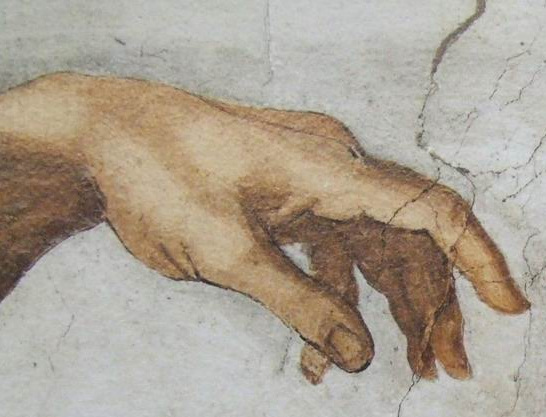
\includegraphics[width=\textwidth]{Adam.jpg}
  \end{frame}

  \begin{frame}
    Popatrz na~swoją dłoń. Każdy punkt twojej dłoni ma 3~współrzędne.
    Te~współrzędne to:
    \begin{itemize}
      \item współrzędna~$x$
      \item współrzędna~$y$
      \item współrzędna~$z$
    \end{itemize}
  \end{frame}

  \begin{frame}
    Matematycy zapisują współrzędne w~słupku:
    $$\g
    \begin{pmatrix}
      x \\
      y \\
      z
    \end{pmatrix}
    $$
    i~mówią na~ten słupek {\g wektor}
  \end{frame}

  \begin{frame}
    Ten wektor ma trzy {\g składowe}:
    $$\g
    \begin{pmatrix}
      x \\
      y \\
      z
    \end{pmatrix}
    $$
  \end{frame}

  \begin{frame}
    Ten wektor ma dwie składowe:
    $$\g
    \begin{pmatrix}
      \hbox{ocena z~języka polskiego} \\
      \hbox{ocena z~matematyki}
    \end{pmatrix}
    $$
  \end{frame}

  \begin{frame}
    Punkty na~tym wykresie oznaczają oceny pięciorga dzieci z~dwóch
    przedmiotów

    \centering
    \begin{tikzpicture}
      \begin{axis}[
          % Zakresy osi od 0 do 6
          xmin=0, xmax=6.5,
          ymin=0, ymax=6.5,
          % Krok siatki co 1 jednostkę
          xtick={1,2,3,4,5,6},
          ytick={1,2,3,4,5,6},
          % Opisy osi
          xlabel={ocena z języka polskiego},
          ylabel={ocena z matematyki},
          grid=both, % Włącza siatkę pomocniczą
          grid style={line width=.1pt, draw=gray!20},
          major grid style={line width=.2pt, draw=gray!50},
          axis lines=left, % Klasyczny wygląd osi (lewa i dolna)
          clip=false % Zapobiega ucinaniu napisów przy krawędziach
        ]
        % Dodanie punktów wraz z etykietami (nodes)
        \addplot[only marks, mark=*, mark size=3pt, myorange] coordinates {
          (4,6) % Orest
          (5,5) % Basia
          (5,4) % Agata
          (4,4) % Jaś
          (6,3) % Marysia
        };
        % Etykiety tekstowe nadpisane bezpośrednio obok punktów, by uniknąć ich najeżdżania na siebie
        \node[above right] at (axis cs:4,6) {Orest (4,6)};
        \node[above right] at (axis cs:5,5) {Basia (5,5)};
        \node[above right] at (axis cs:5,4) {Agata (5,4)};
        \node[below left] at (axis cs:4,4) {Jaś (4,4)};
        \node[above right] at (axis cs:6,3) {Marysia (6,3)};
      \end{axis}
    \end{tikzpicture}
  \end{frame}

  \section{Odwzorowania liniowe}

  \begin{frame}
    Oto odwzorowanie {\g obróć o~$90^\circ$}:
    $$
    \hbox{\g obróć o~$90^\circ$}
\includegraphics[valign=c,width=1cm,height=0.5cm]{uśmiech.png} =
    
\includegraphics[valign=c,width=1cm,height=0.5cm,angle=90,origin=c]{uśmiech.png}
    $$
    Oto odwzorowanie {\g ściśnij}:
    $$
    \hbox{\g ściśnij}
\includegraphics[valign=c,width=1cm,height=0.5cm]{uśmiech.png} =
    
\includegraphics[valign=c,width=1cm,height=0.3cm]{uśmiech.png}
    $$
  \end{frame}

  \begin{frame}
    Oto odwzorowanie {\g obróć o~$90^\circ$ i~ściśnij wynik obrotu}:
    $$ \hbox{\g obróć o~$90^\circ$ i~ściśnij wynik
      obrotu}
\includegraphics[valign=c,width=1cm,height=0.5cm]{uśmiech.png}
    =
    
\includegraphics[valign=c,width=0.6cm,height=0.5cm,angle=90,origin=c]{uśmiech.png}
    $$ Oto odwzorowanie {\g ściśnij i~obróć wynik ściśnięcia
      o~$90^\circ$}:
    $$ \hbox{\g ściśnij i~obróć wynik ściśnięcia
      o~$90^\circ$}
\includegraphics[valign=c,width=1cm,height=0.5cm]{uśmiech.png}
    =
    
\includegraphics[valign=c,width=1cm,height=0.3cm,angle=90,origin=c]{uśmiech.png}
    $$
  \end{frame}

  \begin{frame}
    Żadne z~tych odwzorowań:
    \begin{itemize}
      \item obróć o~$90^\circ$
      \item ściśnij
      \item obróć o~$90^\circ$ i~ściśnij wynik obrotu
      \item ściśnij i~obróć wynik ściśnięcia o~$90^\circ$
    \end{itemize}
    nie krzywi linii prostych
  \end{frame}

  \begin{frame}

    {\g Algebra liniowa} to~nauka o~takich odwzorowaniach, które nie
    krzywią linii prostych
  \end{frame}

  \section{Macierze}

  \begin{frame}

    {\g Macierz} to taka tabela, w której jest przepis na~zmianę
    wektora. Będziemy mówić tylko o~takich macierzach, których
    {\g elementami} są liczby. Oto przykład macierzy:

    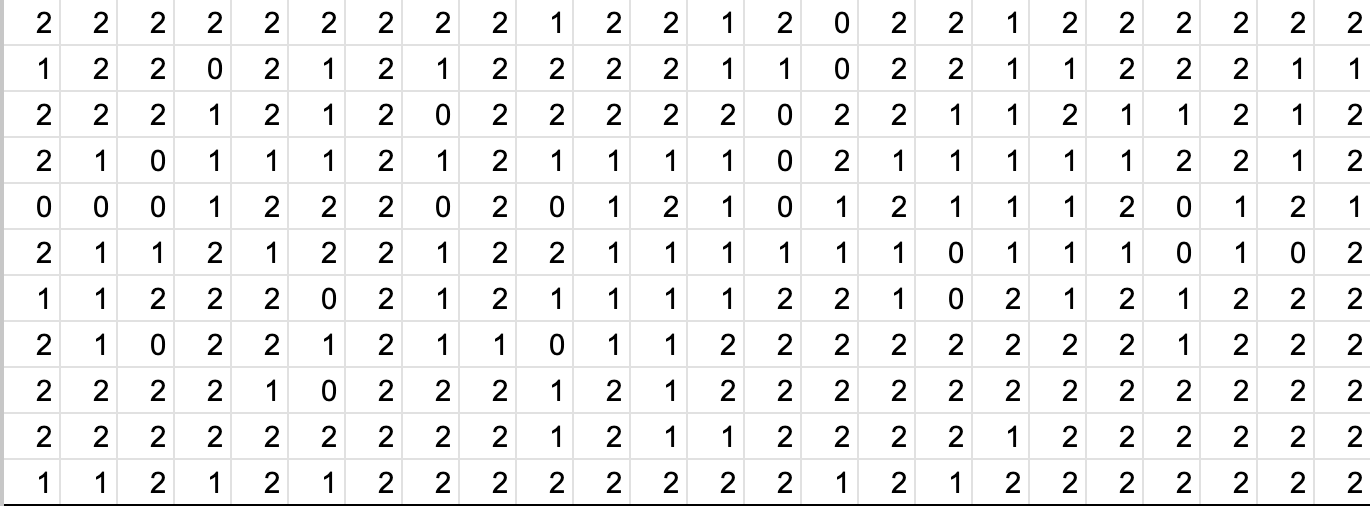
\includegraphics[width=\textwidth]{arkusz.png}
  \end{frame}

  \begin{frame}
    Ta~macierz ma 2~{\g wiersze} i~3~{\g kolumny}:
    $$\g
    \begin{pmatrix}
      1 & 0 & 0 \\
      0 & 1 & 0
    \end{pmatrix}
    $$

    Mówimy, że~ta~macierz ma {\g rozmiar} $2 \times 3$, bo~ma
    2~wiersze i~3~kolumny, ale ta~macierz odwzorowuje wektory
    o~{\g3}~składowych na~wektory o~{\g2}~składowych. Macierze już
    takie są~:-)
  \end{frame}

  \begin{frame}
    Każdy wektor to~też macierz. Macierz o~rozmiarze $N \times 1$.
    Każdy wektor ma $N$~wierszy i~1~kolumnę.
  \end{frame}

  \section{Mnożenie macierzy}

  \begin{frame}
    Aby odwzorować wektor~$X$ na inny wektor~$X'$ odwzorowaniem
    o~nazwie~$A$, mnożymy macierz tego odwzorowania przez wektor~$X$:
    $$\g
    X' = AX
    $$

    To mnożenie to~sposób na~obliczenie, gdzie znajdzie się
    punkt~$X$ po odwzorowaniu~$A$
  \end{frame}

  \begin{frame}
    Tak mnożymy macierz przez wektor:
    $$\g
    \begin{pmatrix}
      1 & 2 & 3 \\
      4 & 5 & 6
    \end{pmatrix}
    \begin{pmatrix}
      x \\
      y \\
      z
    \end{pmatrix} =
    \begin{pmatrix}
      1x + 2y + 3z \\
      4x + 5y + 6z
    \end{pmatrix}
    $$
  \end{frame}

  \begin{frame}
    Przykład: Rzut z przestrzeni trójwymiarowej na~płaszczyznę
    dwuwymiarową.
  \end{frame}

  \begin{frame}
    \centering
    \begin{tikzpicture}[
        % Ustawienie widoku 3D (współrzędne x, y, z w przestrzeni 2D ekranu)
        x={(-0.4cm,-0.5cm)},
        y={(0.9cm,0cm)},
        z={(0cm,0.9cm)},
        scale=1.5,
      ]

      % 1. Rysowanie półprzezroczystej płaszczyzny XY (podłogi) o wymiarach 4x4
      \fill[gray!80, opacity=0.6] (0,0,0) -- (4,0,0) -- (4,4,0) -- (0,4,0) -- cycle;
      % 2. Rysowanie osi układu współrzędnych
      \draw[->, thick, >=Stealth] (0,0,0) -- (4.3,0,0) node[left] {$x$};
      \draw[->, thick, >=Stealth] (0,0,0) -- (0,4.3,0) node[right] {$y$};
      \draw[->, thick, >=Stealth] (0,0,0) -- (0,0,3.3) node[right] {$z$};

      % Podziałki na osiach
      \foreach \val in {1,2,3} {
        \draw (\val,0.05,0) -- (\val,-0.05,0) node[left, scale=0.7] {\val};
        \draw (0.05,\val,0) -- (-0.05,\val,0) node[below, scale=0.7] {\val};
        \draw (0.05,0,\val) -- (-0.05,0,\val) node[right, scale=0.7] {\val};
      }

      % 3. Linie pomocnicze rzutu punktu (pudełko 3D)
      \draw[dashed, gray] (2,0,0) -- (2,3,0) -- (0,3,0);
      \draw[dashed, gray] (2,3,0) -- (2,3,2);
      \draw[dashed, gray] (0,0,2) -- (2,0,2) -- (2,3,2);
      \draw[dashed, gray] (0,0,2) -- (0,3,2) -- (2,3,2);
      \draw[dashed, gray] (2,0,0) -- (2,0,2);
      \draw[dashed, gray] (0,3,0) -- (0,3,2);

      % 4. Definiowanie i oznaczanie punktów
      % Punkt na płaszczyźnie XY (2, 2, 0)
      \fill (2,3,0) circle (1.5pt) node[below right] {$(2,3)$};

      % Punkt w przestrzeni (2, 2, 2)
      \fill (2,3,2) circle (1.5pt) node[above right] {$(2,3,2)$};

      % 5. Połączenie punktów strzałką pionową w dół
      \draw[>=Stealth, ultra thick, orange] (2,3,2) -- (2,3,0);

    \end{tikzpicture}
  \end{frame}

  \begin{frame}
    Rzut z~przestrzeni trójwymiarowej na~płaszczyznę dwuwymiarową.
    $$\g
    A = \begin{pmatrix}
      1 & 0 & 0 \\
      0 & 1 & 0
    \end{pmatrix}
    $$
    $$\g
    X' = \begin{pmatrix}
      1 & 0 & 0 \\
      0 & 1 & 0
    \end{pmatrix}
    \begin{pmatrix}
      x \\
      y \\
      z
    \end{pmatrix} =
    \begin{pmatrix}
      1x + 0y + 0z \\
      0x + 1y + 0z
    \end{pmatrix} =
    \begin{pmatrix}
      x \\
      y
    \end{pmatrix}
    $$
  \end{frame}

  \begin{frame}
    Każdemu odwzorowaniu liniowemu odpowiada macierz
  \end{frame}

  \begin{frame}
    Odwzorowanie {\g ściśnij}:
    \centering
    \begin{tikzpicture}[scale=1.5]
      % Osie współrzędnych
      \draw[=>Stealth, thick] (-0.5, 0) -- (3.5, 0) node[right] {$x$};
      \draw[=>Stealth, thick] (0, -0.5) -- (0, 3.5) node[above] {$y$};

      % Podziałka na osiach
      \foreach \x in {1, 2, 3}
      \draw (\x, 2pt) -- (\x, -2pt) node[below] {$\x$};
      \foreach \y in {1, 2, 3}
      \draw (2pt, \y) -- (-2pt, \y) node[left] {$\y$};
      \node[below left] at (0, 0) {$0$};

      % Linie pomocnicze (przerywane)
      \draw[gray, dotted] (2, 0) -- (2, 2) -- (0, 2);
      \draw[gray, dotted] (0, 1) -- (2, 1);

      % Punkty
      \fill (2, 2) circle (2pt) node[above right] {$(2,2)$};
      \fill (2, 1) circle (2pt) node[below right] {$(2,1)$};

      % Strzałka z (2,2) do (2,1)
      \draw[=>Stealth, ultra thick, myorange] (2, 2) -- (2, 1);
    \end{tikzpicture}
  \end{frame}

  \begin{frame}
    $$\g
    \hbox{ściśnij} = \begin{pmatrix}
      1 & 0 \\
      0 & 0{,}5
    \end{pmatrix}
    $$
    bo
    $$\g
    \begin{pmatrix}
      1 & 0 \\
      0 & 0{,}5
    \end{pmatrix}
    \begin{pmatrix}
      x \\
      y
    \end{pmatrix} =
    \begin{pmatrix}
      1x + 0y \\
      0x + 0{,}5y
    \end{pmatrix} =
    \begin{pmatrix}
      x \\
      0{,}5y
    \end{pmatrix}
    $$
  \end{frame}

  \begin{frame}
    Odwzorowanie {\g obróć o~$90^\circ$}:
    \centering
    \begin{tikzpicture}[scale=0.8]
      % Osie współrzędnych
      \draw[=>Stealth, thick] (-4.5, 0) -- (4.5, 0) node[right] {$x$};
      \draw[=>Stealth, thick] (0, -2.5) -- (0, 4.5) node[above] {$y$};

      % Podziałki i opis osi
      \foreach \x in {-4,-3,-2,-1,1,2,3,4}
      \draw (\x, 2pt) -- (\x, -2pt) node[below, font=\small] {$\x$};
      \foreach \y in {-2,-1,1,2,3,4}
      \draw (2pt, \y) -- (-2pt, \y) node[left, font=\small] {$\y$};
      \node[below left] at (0, 0) {$0$};

      % Punkty
      \fill (2, 3) circle (2pt) node[above right] {$(2,3)$};
      \fill (-3, 2) circle (2pt) node[above left] {$(-3,2)$};

      % Linie pomocnicze (przerywane)
      \draw[gray, dotted] (2, 0) -- (2, 3) -- (0, 3);
      \draw[gray, dotted] (-3, 0) -- (-3, 2) -- (0, 2);

      % Ćwierćokrągła strzałka o środku w (0,0)
      % Kąt początkowy: atan2(3,2), promień: sqrt(2^2 + 3^2) = sqrt(13), kąt łuku: 90°
      \draw[=>Stealth, ultra thick, myorange] (2,3) arc[
        start angle={atan2(3,2)},
        delta angle=90,
        radius={veclen(2,3)}
      ];
    \end{tikzpicture}
  \end{frame}

  \begin{frame}
    $$\g
    \hbox{obróć o~$90^\circ$} = \begin{pmatrix}
      0 & -1 \\
      1 & 0
    \end{pmatrix}
    $$
    bo
    $$\g
    \begin{pmatrix}
      0 & -1 \\
      1 & 0
    \end{pmatrix}
    \begin{pmatrix}
      x \\
      y
    \end{pmatrix} =
    \begin{pmatrix}
      0x + -1y \\
      1x + 0y
    \end{pmatrix} =
    \begin{pmatrix}
      -y \\
      x
    \end{pmatrix}
    $$
  \end{frame}

  \begin{frame}
    Każdą macierz możemy traktować jako zestaw wektorów. Każdy z~tych
    wektorów zajmuje jedną kolumnę macierzy. Na~przykład:
    $$\g
    A = \begin{pmatrix}
      \color{myred} 1 & \color{myorange} 0 & \color{myblue} 0 \\
      \color{myred} 0 & \color{myorange} 1 & \color{myblue} 0
    \end{pmatrix}
    $$
  \end{frame}

  \begin{frame}
    Tak mnożymy macierz przez macierz:\\Lewym palcem idziemy w~prawo
    po~wierszu, a~prawym w~dół po~kolumnie. Mnożymy napotkane pary
    i~dodajemy wyniki. Na~przykład:
    $$
    \begin{pmatrix}
      \color{myred}1 & \color{myorange}2 & \color{myblue}3 & \color{mygreen}4 \\
      \color{myred}5 & \color{myorange}6 & \color{myblue}7 & \color{mygreen}8
    \end{pmatrix}
    \begin{pmatrix}
      \color{myred}a & \color{myred}e & \color{myred}i \\
      \color{myorange}b & \color{myorange}f & \color{myorange}j \\
      \color{myblue}c & \color{myblue}g & \color{myblue}k \\
      \color{mygreen}d & \color{mygreen}h & \color{mygreen}l
    \end{pmatrix} = {}
    $$
    $$
    {} = \begin{pmatrix}
      {\color{myred}1a}+{\color{myorange}2b}+{\color{myblue}3c}+{\color{mygreen}4d}&
      {\color{myred}1e}+{\color{myorange}2f}+{\color{myblue}3g}+{\color{mygreen}4h}&
      {\color{myred}1i}+{\color{myorange}2j}+{\color{myblue}3k}+{\color{mygreen}4l}\\
      {\color{myred}5a}+{\color{myorange}6b}+{\color{myblue}7c}+{\color{mygreen}8d}&
      {\color{myred}5e}+{\color{myorange}6f}+{\color{myblue}7g}+{\color{mygreen}8h}&
      {\color{myred}5i}+{\color{myorange}6j}+{\color{myblue}7k}+{\color{mygreen}8l}
    \end{pmatrix}
    $$
  \end{frame}

  \begin{frame}
    W mnożeniu macierzy obowiązuje zasada zgodności ich rozmiarów.
    Na~przykład:
    $$
    (\hbox{macierz } {\color{myorange}2} \times {\color{mygreen}4})\cdot
    (\hbox{macierz } {\color{mygreen}4} \times {\color{myorange}3}) =
    \hbox{macierz } {\color{myorange}2} \times {\color{myorange}3}
    $$

    Liczby, które są w~środku ({\color{mygreen}4}
    i~{\color{mygreen}4}) muszą być takie same

    Wynik mnożenia ma rozmiar wyznaczony przez liczby z~brzegu
    ({\color{myorange}2} i~{\color{myorange}3})
  \end{frame}

  \begin{frame}
    Tak dodajemy i~odejmujemy macierze. Obie macierze muszą mieć taki
    sam rozmiar, czyli tyle samo wierszy i~tyle samo kolumn.
    $$\g
    \begin{pmatrix}
      1 & 4 \\
      2 & 5 \\
      3 & 6
    \end{pmatrix} +
    \begin{pmatrix}
      3 & 3 \\
      0 & 1 \\
      2 & 1
    \end{pmatrix} =
    \begin{pmatrix}
      1+3 & 4+3 \\
      2+0 & 5+1 \\
      3+2 & 6+1
    \end{pmatrix} =
    \begin{pmatrix}
      4 & 7 \\
      2 & 6 \\
      5 & 7
    \end{pmatrix}
    $$
    $$\g
    \begin{pmatrix}
      2 & 1 \\
      1 & 2
    \end{pmatrix} -
    \begin{pmatrix}
      2 & 2 \\
      0 & 1
    \end{pmatrix} =
    \begin{pmatrix}
      2-2 & 1-2 \\
      1-0 & 2-1
    \end{pmatrix} =
    \begin{pmatrix}
      0 & -1 \\
      1 & 1
    \end{pmatrix}
    $$
  \end{frame}

  \section{Rozkład na~wartości osobliwe (SVD)}

  \begin{frame}{Dane wejściowe}
    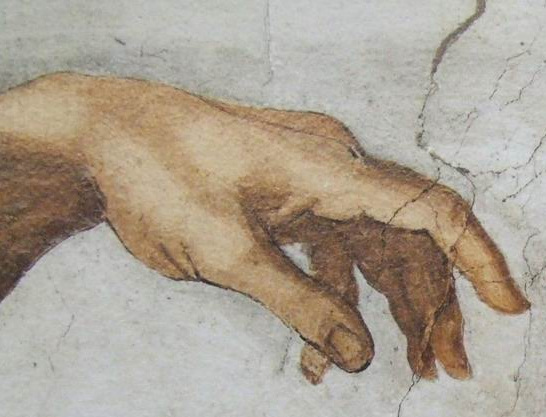
\includegraphics[width=\textwidth]{Adam.jpg}
  \end{frame}

  \begin{frame}{Dane wejściowe}
    Znów popatrz na~swoją dłoń. Wyprostuj palce i~obróć swoją dłoń,
    jak chcesz. Wyobraź sobie, że~twoja dłoń to~chmura tysięcy punktów
    w~przestrzeni trójwymiarowej.
  \end{frame}

  \begin{frame}{Obrót osi}
    Wektor $\begin{pmatrix}3 \\ 2\end{pmatrix}$ to~instrukcja ruchu:
      zrób 3~kroki na~wschód i~2~kroki na~północ. Ale {\g
        zachód-wschód} i~{\g południe-północ} to~tylko umowne osie.
      Gdy obrócimy mapę, ten sam ruch będą opisywać inne liczby.
  \end{frame}

  \begin{frame}{Obrót osi}
    Zamiast opisywać położenie punktów w~układzie współrzędnych
    związanym ze~ścianami pokoju ({dół-góra}, {lewo-prawo},
    {tył-przód}), {\g rozkład~na~wartości osobliwe} ({\g
      Singular~Value~Decomposition}, czyli {\g SVD}) obraca osie tak,
    aby dopasować je do~naturalnego kształtu dłoni.
  \end{frame}

  \begin{frame}{Prawe wektory osobliwe}
    \begin{itemize}
      \item {\g pierwszy prawy wektor osobliwy} wskazuje kierunek
        od~nadgarstka do~środkowego palca
      \item {\g drugi prawy wektor osobliwy} wskazuje kierunek
        od~kciuka do~małego palca
      \item {\g trzeci prawy wektor osobliwy} wskazuje kierunek
        od~wnętrza dłoni do~jej grzbietu
    \end{itemize}
  \end{frame}

  \begin{frame}{Prawe wektory osobliwe}
    Każdy z~tych trzech wektorów jest prostopadły do~wszystkich
    pozostałych wektorów.

    W~SVD zawsze tak jest~:-)
  \end{frame}

  \begin{frame}{Wartości osobliwe}
    Wartości osobliwe mierzą to, jak bardzo chmura punktów jest
    rozciągnięta wzdłuż nowych osi:
    \begin{itemize}
      \item {\g pierwsza wartość osobliwa} (duża) odpowiada dużemu
        rozrzutowi punktów wzdłuż długości dłoni
      \item {\g druga wartość osobliwa} (średnia) odpowiada rozrzutowi
        punktów wzdłuż szerokości dłoni
      \item {\g trzecia wartość osobliwa} (mała) odpowiada małemu
        rozrzutowi punktów wzdłuż grubości dłoni
    \end{itemize}
  \end{frame}

  \begin{frame}{Lewe wektory osobliwe}
    Podczas gdy prawe wektory osobliwe opisują naturalny kształt dłoni
    w~powietrzu, lewe wektory osobliwe opisują układ współrzędnych,
    do~którego przenosimy ten kształt.

    Lewe wektory osobliwe wskazują, jak należy obrócić obraz dłoni,
    aby dłoń ukazała się nam w~najbardziej naturalnym położeniu.
  \end{frame}

  \begin{frame}{Dlaczego SVD jest fajne?}
    SVD jest fajne, bo~gdy pewne wartości osobliwe są bliskie zeru,
    te~wektory osobliwe, które im odpowiadają, niosą nieistotne
    szczegóły lub szum. Wtedy możemy wyzerować te~wartości osobliwe
    i~pominąć te~wektory osobliwe.
  \end{frame}

  \begin{frame}{Zerujemy wartości osobliwe}
    Gdy wyzerujemy trzecią wartość osobliwą, spłaszczymy chmurę
    punktów wzdłuż osi grubości. Zamiast bryły~3D otrzymamy płaski,
    dwuwymiarowy płat.

    Ponieważ grubość dłoni jest niewielka, po~tym spłaszczeniu
    zachowujemy prawie 100\% oryginalnego kształtu i~proporcji dłoni,
    pozbywając się najmniej istotnego wymiaru.
  \end{frame}

  \begin{frame}
    Każde dziecko wie, że~dłoń najlepiej widać, gdy narysuje się ją
    tak, że~widać jej długość i~szerokość~:-)

    \centering
    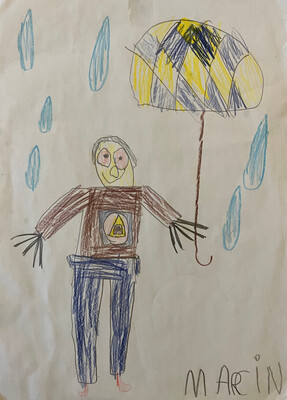
\includegraphics[height=0.85\textheight]{Marcin.jpg}
  \end{frame}

  \begin{frame}{SVD jako mnożenie macierzy}
    SVD polega na~tym, że~każde odwzorowanie liniowe przestrzeni
    $n$-wymiarowej w~przestrzeń $m$-wymiarową to~3~działania
    wykonywane po~kolei:

    {\g obrót/odbicie $\to$ rozciąganie/ściskanie $\to$ obrót/odbicie}
  \end{frame}

  \begin{frame}{SVD jako mnożenie macierzy}
    {\g obrót/odbicie $\to$ rozciąganie/ściskanie $\to$ obrót/odbicie}

    Tym trzem odwzorowaniom odpowiada mnożenie 3~macierzy:

    {\g macierz~$m \times n$ =\\= macierz~$m \times m$
    $\cdot$ macierz~$m \times n$
    $\cdot$ macierz~$n \times n$}

    Gdy mnożymy macierz przez wektor, wektor stoi po~prawej stronie,
    dlatego pierwsze działanie wykonuje macierz stojąca najbardziej
    po~prawej.
  \end{frame}

  \begin{frame}{SVD jako mnożenie macierzy}

    {\g macierz~$m \times m$
    $\cdot$ macierz~$m \times n$
      $\cdot$ macierz~$n \times n$}

    \begin{itemize}
      \item Obrót lub odbicie przestrzeni danych: opisują to liczby
        w~macierzy~$\g n \times n$. Są~to {\g prawe wektory osobliwe}
        tego odwzorowania.
      \item Rozciąganie/ściskanie: Liczby na~przekątnej macierzy~$\g m
        \times n$ to~{\g wartości osobliwe} tego odwzorowania.
        Określają skalowanie wektorów osobliwych.
      \item Obrót lub odbicie przestrzeni docelowej: opisują to liczby
        w~macierzy~$\g m \times m$. Są~to~{\g lewe wektory osobliwe}
        tego odwzorowania.
    \end{itemize}
  \end{frame}

  \section{Analiza głównych składowych (PCA)}

  \begin{frame}
    Zamiast przeprowadzać zwykły rozkład~SVD, lepiej jest:
    \begin{itemize}
      \item odjąć od~każdej współrzędnej średnią wartość tej
        współrzędnej we~wszystkich kolumnach, aby przesunąć dane
        ku~zeru
      \item przeprowadzić na~tak przygotowanej macierzy rozkład~SVD
      \item (opcjonalnie) odrzucić te~wektory osobliwe, którym
        odpowiadają małe wartości osobliwe
    \end{itemize}
    Taka procedura to~{\g analiza głównych składowych} ({\g Principal
      Component Analysis}, czyli~{\g PCA})
  \end{frame}

  \begin{frame}
    \begin{tikzpicture}[scale=1.8, >=stealth]
      % Siatka pomocnicza
      \draw[gray!15, very thin, step=0.5] (-2.3, -1.2) grid (2.3, 1.2);

      % Osie układu współrzędnych
      \draw[->, thick] (-2.4, 0) -- (2.4, 0) node[right] {$x$};
      \draw[->, thick] (0, -1.3) -- (0, 1.3) node[above] {$y$};

      % Podziałki na osiach
      \foreach \x in {-2, -1, 1, 2}
      \draw (\x, 0.04) -- (\x, -0.04) node[below, font=\tiny, inner sep=1pt] {\x};
      \foreach \y in {-1, 1}
      \draw (0.04, \y) -- (-0.04, \y) node[left, font=\tiny, inner sep=1pt] {\y};

      \node[below left, font=\tiny] at (0,0) {$0$};

      % Styl punktów
      \tikzset{
        point/.style={circle, fill=myorange, inner sep=1.5pt},
        label/.style={font=\small, inner sep=3pt}
      }

      % Punkty z opisami
      \node[point] (Orest)   at (1.77889962,  0.18845726) {};
      \node[label, above right] at (Orest) {Orest (4, 6)};

      \node[point] (Basia)   at (0.39761059,  0.49183922) {};
      \node[label, above]       at (Basia) {Basia (5, 5)};

      \node[point] (Agata)   at (-0.44472491, -0.04711431) {};
      \node[label, below left]  at (Agata) {Agata (5, 4)};

      \node[point] (Jas)     at (0.09422863, -0.88944981) {};
      \node[label, right]       at (Jas) {Jaś (4, 4)};

      \node[point] (Marysia) at (-1.82601394,  0.25626765) {};
      \node[label, above left]  at (Marysia) {Marysia (6, 3)};

    \end{tikzpicture}
    Oś~$x$ odpowiada uzdolnieniom humanistycznym-ścisłym

    Oś~$y$ odpowiada ogólnym uzdolnieniom
  \end{frame}

\end{document}
